%\documentclass{article}

%\usepackage[utf8]{inputenc}
\usepackage{placeins}
\usepackage{graphicx}
\usepackage[ruled,vlined,linesnumbered]{algorithm2e}
\usepackage{listings}
\usepackage{amsthm}
\usepackage{amsmath}
\usepackage{caption}
\usepackage{epigraph}

\captionsetup[figure]{font=scriptsize}

\newtheorem{definition}{Definição}[section]
\theoremstyle{remark}
\newtheorem*{remark}{Observações}
\theoremstyle{theorem}
\newtheorem{theorem}{Teorema}[section]

\setlength{\parskip}{.5em}

\renewcommand\refname{Leituras adicionais}
\renewcommand\figurename{Figura}
\renewcommand{\lstlistingname}{Código}

\newcommand{\eclipse}{$ECL^iPS^e$}
\newcommand{\definicao}[1]{\textbf{#1}\marginpar{\small \textbf{#1}}}

\lstdefinestyle{prosty}{
  language=Prolog,
  basicstyle=\small
}



\usetikzlibrary{shapes.geometric, arrows} \tikzstyle{decision} =
               [diamond, minimum width=1cm, minimum height=1cm, text
                 centered, draw=black, fill=green!30]
               \tikzstyle{arrow} = [thick,->,>=stealth]

%\begin{document}
\section{Restrições}

Como vimos anteriormente, uma das ideias iniciais da programação
lógica era de permitir à programadora expressar \enphasis{o que} o
programa faz, sem ter que se preocupar muito em \enphasis{como} ele o
faz, o que fazemos expressando a lógica do programa em termos de
relações. Na maior parte dos paradigmas de programação usuais, há uma
dificuldade em expressar essas relações, ou
restrições\footnote{Estarmos tratando relação como sinônimo a
  restrição é um abuso de linguagem usado aqui por sua conveniência,
  mas é importante lembrar que são coisas diferentes.}, entre os
objetos definidos no programa.

Com a programação lógica, isso é um pouco aliviado. Por exemplo, se
soubermos a gramática do Prolog, não é difícil ler o programa Member
(copiado a seguir, para referência) como expressando uma relação que
existe entre um termo X e um Xs se Xs puder ser escrito como
\codigo{[X|Xs]} ou, se for possível escrever Xs como \codigo{[Y|Ys]} e
X tiver a relação member com Ys.

\begin{listing}
  \inputminted{prolog}{../Exemplos/Cap4/prog1_member.pl}
  \caption{Member}
\end{listing}

Mas vimos também que operações aritméticas, no Prolog, não funcionam
de maneira relacional (ao fazermos uma soma, por exemplo, o ``+''
funciona como uma função, retornando um valor, no lugar de como uma
restrição ou relação). Isso é grave, porque expressões aritméticas
aparecem de várias formas em problemas reais e não ser capaz de
expressá-las relacionalmente poderia levar a um código muito maior,
redundante e difícil de manter.

Para se convencer disso, considere, como um exemplo, a equação da lei
de Ohm: I = V/R (onde I é a corrente, V a tensão e R a resistência).
Claramente, essa equação expressa a relação entre I, V e R, assim como
as restrições provenientes dessa relação, indicando que, fixando
quaisquer duas das variáveis, a terceira também é fixada e, fixando
uma, as duas outras obedecem a uma restrição (por exemplo, se V = 10
volts, temos que $I \times R$ = 10). Atualmente, não conseguimos
expressar esse tipo de relação em código sem algum esforço.

Vimos uma forma limitada de lidarmos com isso no Capítulo anterior,
%TODO Adicionar ref para Capítulo
mas precisaremos de algo mais poderoso se quisermos lidar com
problemas mais complexos. Antes disso, 
será útil nos abstrairmos um pouco disso para vermos a programação por
restrições de uma forma mais ampla.

\subsection{Domínios}

Restrições não se limitam a restrições aritméticas. Existem vários
tipos de restrições, cada uma possivelmente agindo em diferentes
domínios.  O domínio é o que determina as formas legítimas de
restrição e o que elas significam. Restrições são escritas usando
constantes (como 0, ou 1) e símbolos que agem como funções (como ``+''
ou ``-''). O domínio determina a sintaxe das restrições: quais
símbolos de restrições podem ser usados, quais e quantos são os
argumentos de cada símbolo e a ordem em que são escritos.

Dois exemplos de domínios que conhecemos são o dos Reais e o dos
Inteiros, com os símbolos de restrições usuais (isto é: ``+'',
``$<$'', etc.). Outros exemplos de domínios são o das Árvores e o dos
Booleanos. São domínios de grande importância e, por isso,
discorreremos momentaneamente um pouco sobre eles logo mais. Em se
tratando de domínios aritméticos, a não ser quando dito o contrário,
assumiremos que lidamos com o domínio dos Reais.

Definido o domínio, dada uma restrição, precisamos saber o que
queremos dela. Algumas das opções mais comuns são:
\begin{enumerate}
\item Checar se a restrição é satisfazível (isto é, se existe
  alguma substituição para a qual a restrição é verdadeira);
\item Encontrar uma substituição que respeite as restrições;
\item Otimizar a substituição encontrada por meio de uma função
  (comumente chamada \enphasis{função custo} (apesar de muitas
  vezes não podermos interpretar essa função como algum ``custo''
  de forma natural)).
\end{enumerate}

Claramente, se conseguimos (2), conseguimos (1) e, se conseguimos
(2), conseguimos (1) e (2). Frequentemente, conseguir (1) será
equivalente a conseguir (2), porque seguimos um método
construtivo. Nem sempre, no entanto, conseguiremos (1). Sabemos, por
exemplo, que no domínio dos Inteiros existem restrições que não se
sabe se podem ser satisfeitas.

Ou talvez possamos, a princípio, dizer se a restrição em um domínio
seja satisfazível, mas na prática isso se torne computacionalmente
inviável se a restrição for muito complicada ou complexa. O problema
de descobrir se uma restrição booleana pode ou não ser satisfeita
(mais conhecido como SAT, de \foreign{Propositional Satisfiability
  Testing}), é um famoso problema NP-difícil e ainda hoje um tema de
ativa pesquisa (veja, por exemplo, \cite{sat}).

Esse tipo de constatação rápida já nos dá uma ideia do tipo de
pergunta que precisaríamos fazer dado um domínio, assim como da
variedade de tipos de restrição que existem, mesmo em um domínio.

Daqui para frente denotaremos problemas de otimização como COP (de
\foreign{Constraint Optimization Problem}), de satisfação de
restrições como CSP (de \foreign{Constraint Satisfaction Problem}) e,
quando não for necessário fazer distinção, apenas CP. Até agora, temos
lidado com CPs como contendo uma restrição, mas será conveniente lidar
com eles como contendo uma conjunção de restrições:

Se $x_0$ é um símbolo de restrição no domínio, junto de seus
argumentos, diremos que é uma \definicao{restrição primitiva}. Uma
\definicao{restrição composta} C é a conjunção de restrições
primitivas: $x_0$, ..., $x_n$ (em que as vírgulas, como usual, são
lidas como um \technical{e} lógico), em que $x_i$ é uma restrição
primitiva. Assim, um COP é descrito por uma tupla (C, f), enquanto que
um CSP é descrito por algum C, em que C é uma restrição
composta. Daqui para frente nos referiremos a uma substituição nas
variáveis de um CP que respeite às restrições como uma solução desse
CP.

\subsection{Árvores}
Como você logo perceberá (ou talvez já o tenha percebido), já vimos
restrições por árvores antes, elas só estavam um pouco disfarçadas.

Um \definicao{construtor de árvore} é uma sequência de caracteres
começando com um caractere minúsculo. Definimos uma árvore
recursivamente como: uma constante é uma árvore (de altura 1); um
construtor de árvore com um conjunto de n $\geq$ 1 árvores é uma
árvore.

Árvores são comumente representadas na forma de diagramas como os
seguintes:

\Tree[.cons 1 [.cons 2 [.cons 3 4 ] ] ]

ou

\Tree[ .{café da manhã} [.café canela açúcar ] {pão de queijo} [.pão
    queijo ] goiabada ]

Que podem ser reescritos, de forma mais compacta como \codigo{cons(1,
  cons(2, cons(3, 4)))}\footnote{A leitora de olhos afiados vai notar
  que é mais ou menos assim que representamos listas, trocando o
  ``cons'' pelo ``.''.} e \codigo{café da manhã(café(canela, açúcar),
  pão de queijo, pão(queijo), goiabada)}\footnote{Estamos usando
  caracteres especiais aqui para fins de expressividade, mas seu uso
  em códigos de computador deve ser evitado.}.  Como pode ver, é
essencialmente a mesma representação que temos para um funtor (junto
com seus argumentos): funtores são árvores, árvores são funtores
(neste contexto).

Um algoritmo muito próximo ao algoritmo de unificação, que vimos no
Capítulo 1 %TODO adicionar link
, serve para resolver restrições em
árvore do tipo $T_1$ = $T_2$, em que $T_1$ e $T_2$ são árvores. É
interessante notar que um algoritmo para resolução de restrições em
árvores foi dado por Herbrand\cite{herbrand} de forma independente ao
do algoritmo de unificação de Robinson.

Vale notar também outro detalhe importante naquele algoritmo: ele
realiza um procedimento que frequentemente fazemos ao buscar resolver
um problema, isto é, transformando uma pergunta, potencialmente
complicada e difícil, em uma trivial, para a qual sabe-se a
resposta. Essa é uma instância de um processo de
\definicao{normalização}, isto é, um processo de transformar uma
restrição em outra equivalente, mas mais tratável. Processos de
normalização frequentemente exercem um papel importante. Voltaremos a
esse tema depois.

\subsection{Ideias de resolução}

Nossa discussão sobre problemas envolvendo restrições até agora foi
uma discussão geral e apesar de muitas vezes, para resolver esses
problemas, ser preferível usar métodos específicos ao domínio e ao
tipo de problema, muitas vezes esses problemas são heterogêneos o
suficiente para não permitir isso ou não fazem uso de uma sintaxe que
permita o uso de métodos específicos.  É útil então termos alguma ou
algumas formas gerais de resolver esses problemas. Eles são baseados
em busca.

\subsubsection{Propagação local}

Propagação local é melhor explicada por um desenho. O grafo a seguir
representa a modelagem de um circuito elétrico.  As ``caixinhas''
representam as relações de restrições e as ``bolinhas'', os dados ou
variáveis. Por exemplo, uma ``caixinha'' com sinal de adição indica
que os dados (no caso, as variáveis) que entram por ela (o que é
indicado pela seta) somadas devem ser iguais às variáveis, ou dados,
de saída (indicado por outra seta).

\begin{center}
  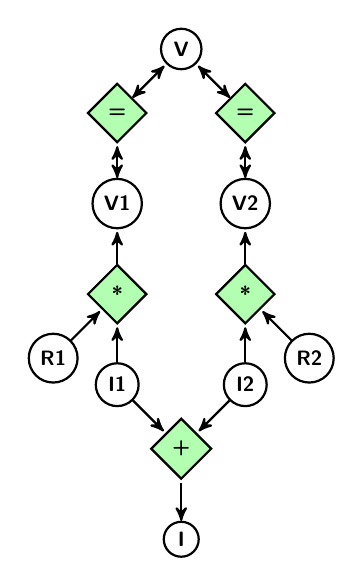
\begin{tikzpicture}[->,>=stealth',shorten >=1pt,auto,node distance=1.15cm, thick,main node/.style={circle,draw,font=\sffamily\bfseries}]

    \node[main node] (V) [scale=0.75]{V}; \node[main node] (eq)
         [decision, below left of=V, scale=0.75] {=}; \node[main node]
         (eq1)[decision, below right of=V, scale=0.75] {=}; \node[main
           node] (V1) [below of= eq, scale=0.75] {V1}; \node[main
           node] (V2) [below of= eq1, scale=0.75] {V2}; \node[main
           node] (tm) [decision, below of=V1, scale=0.75] {*};
         \node[main node] (tm1)[decision, below of=V2, scale=0.75]
              {*}; \node[main node] (R1) [below left of=tm,
                scale=0.75] {R1}; \node[main node] (R2) [below right
                of=tm1, scale=0.75] {R2}; \node[main node] (I1) [below
                of=tm, scale=0.75] {I1}; \node[main node] (I2) [below
                of=tm1, scale=0.75] {I2}; \node[main node]
              (pls)[decision, below right of=I1, scale=0.75] {+};
              \node[main node] (I) [below of=pls, scale=0.75] {I};

              \draw [thick,<->] (eq) -- (V); \draw [thick,<->] (eq1) -- (V);
              \draw [thick,<->] (V1) -- (eq); \draw [thick,<->] (V2) -- (eq1);
              \draw [thick,->] (R1) -- (tm); \draw [thick,->] (I1) -- (tm);
              \draw [thick,->] (tm) -- (V1); \draw [thick,->] (tm1) -- (V2);
              \draw [thick,->] (I2) -- (tm1); \draw [thick,->] (R2) -- (tm1);
              \draw [thick,->] (I1) -- (pls); \draw [thick,->] (I2) -- (pls);
              \draw [thick,<-] (I) -- (pls);

              %\path[every node/.style={font=\sffamily\small}] (1) edge node
              %[left] {0.6} (4) edge [bend right] node[left] {0.3} (2) edge
              %[loop above] node {0.1} (1) (2) edge node [right] {0.4} (1)
              %edge node {0.3} (4) edge [loop left] node {0.4} (2) edge [bend
              %right] node[left] {0.1} (3) (3) edge node [right] {0.8} (2)
              %edge [bend right] node[right] {0.2} (4) (4) edge node [left]
              %{0.2} (3) edge [loop right] node {0.6} (4) edge [bend right]
              %node[right] {0.2} (1);
  \end{tikzpicture}
\end{center}


Esse grafo é uma outra forma de representar a restrição \codigo{V=V1,
  V=V2, V1=I1*R1, V2=I2*R2, I=I1+I2}\footnote{Exemplo adaptado de
  \cite{marriot}, pág. 36.}. Considere as restrições adicionais de que
\codigo{V=8, R1=6, R2=44}. Na propagação local, podemos considerar as
arestas como veículos das restrições, deixando-as passar de nó em nó
de forma apropriada, passo a passo. Por exemplo, dadas as restrições
acima, a restrição de \codigo{V=8} pode ser propagada para
\codigo{V1=8}, e teríamos:


\begin{center}
  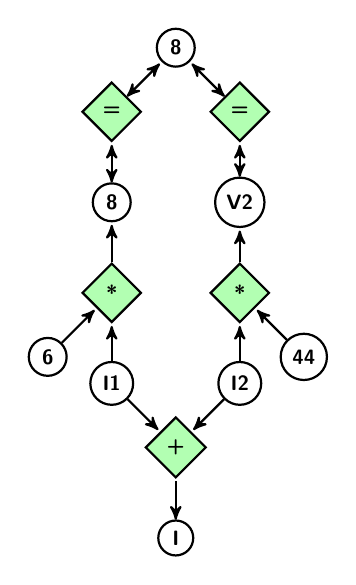
\begin{tikzpicture}[->,>=stealth',shorten >=1pt,auto,node distance=1.15cm, thick,main node/.style={circle,draw,font=\sffamily\bfseries}]

    \node[main node] (V) [scale=0.75]{8}; \node[main node] (eq)
         [decision, below left of=V, scale=0.75] {=}; \node[main node]
         (eq1)[decision, below right of=V, scale=0.75] {=}; \node[main
           node] (V1) [below of= eq, scale=0.75] {8}; \node[main node]
         (V2) [below of= eq1, scale=0.75] {V2}; \node[main node] (tm)
         [decision, below of=V1, scale=0.75] {*}; \node[main node]
         (tm1)[decision, below of=V2, scale=0.75] {*}; \node[main
           node] (R1) [below left of=tm, scale=0.75] {6}; \node[main
           node] (R2) [below right of=tm1, scale=0.75] {44};
         \node[main node] (I1) [below of=tm, scale=0.75] {I1};
         \node[main node] (I2) [below of=tm1, scale=0.75] {I2};
         \node[main node] (pls)[decision, below right of=I1,
           scale=0.75] {+}; \node[main node] (I) [below of=pls,
           scale=0.75] {I};

         \draw [thick,<->] (eq) -- (V); \draw [thick,<->] (eq1) -- (V);
         \draw [thick,<->] (V1) -- (eq); \draw [thick,<->] (V2) -- (eq1);
         \draw [thick,->] (R1) -- (tm); \draw [thick,->] (I1) -- (tm);
         \draw [thick,->] (tm) -- (V1); \draw [thick,->] (tm1) -- (V2);
         \draw [thick,->] (I2) -- (tm1); \draw [thick,->] (R2) -- (tm1);
         \draw [thick,->] (I1) -- (pls); \draw [thick,->] (I2) -- (pls);
         \draw [thick,<-] (I) -- (pls);

  \end{tikzpicture}
\end{center}

Disso, podemos continuar a propagação, obtendo \codigo{I1 = 8/6}. E
assim vai.

Propagação local funciona muito bem para resolver alguns problemas,
mas simplesmente não consegue resolver outros. Por exemplo, considere
a restrição \codigo{A=B+2*Z, A=3*K-B, K=5, Z=7}. Propagação local
detectaria que \codigo{K=5} e \codigo{Z=7}, mas não encontraria o
valor de A ou B. Isso ocorre porque para tanto seria preciso fazer uso
de mais de uma restrição por vez, o que a propagação local não faz.

Mais geralmente, dizemos que um \definicao{propagador} é uma função
monotônica não-crescente de domínio para domínio, i.e. se \enphasis{D}
e \enphasis{D'} são domínios tais que $D \subseteq D'$ e \enphasis{f}
é um propagador, obrigatoriamente $f(D') \subseteq f(D)$ e $f(D)
\subseteq D$. Um propagador é dito correto em relação a uma restrição
\funtor{r/n} com variáveis de domínios $D_i$ se as soluções para a
restrição nos domínios originais são as mesmas que as soluções para a
restrição em $f(D_i)$.  Perceba que essa é uma noção fraca, já que a
função identidade a satisfaz. Propagação local é um tipo de propagador
correto (veremos outros mais para frente). No frigir dos ovos, o que
um propagador faz impedir que o resolvedor teste todas as
possibilidades descartando algumas possibilidades que não dariam
certo.

No geral, em um CSP, provê-se um propagador para cada restrição. Nesse
contexto, um \definicao{resolvedor por propagação} para um conjunto de
propagadores \enphasis{P} aplica os propagadores em \enphasis{P} a
cada restrição até que não haja mudanças a serem obtidas. Em outras
palavras, um resolvedor \enphasis{solv} por propagação recebe como
argumentos um conjunto de propagadores \enphasis{P} e um de restrições
\enphasis{R} e retorna um conjunto de domínios que é o maior ponto
fixo dos propagadores em \enphasis{P} com respeito à relação de
inclusão (assumindo que tal conjunto de domínios exista, o que
geralmente é o caso).

\subsection{Busca Top-Down}

Propagação local pode ser uma técnica muito útil para resolver alguns
problemas, e pode ficar mais poderosa ainda se combinada com uma
estratégia de \enphasis{ramificação}. A essa combinação chamaremos de
busca \foreign{top-down}.

Intuitivamente, a propagação de restrições ajuda a transformar o
problema em outro mais simples. O passo de ramificação serve, então,
para partir o problema em problemas menores, aos quais poderemos
aplicar a propagação de restrições novamente, seguido por outra
ramificação, e assim vai, gerando uma árvore de busca. A forma padrão
de busca top-down é chamada de \definicao{busca por
  backtracking}. Essa forma de busca funciona simplesmente gerando a
dita árvore e fazendo a travessia dela (frequentemente, faremos a
travessia enquanto geramos a árvore, não depois). Vale notar que, na
presença de propagação de restrições, ocasionalmente pode ser útil
adicionar à escrita do problema restrições implícitas, que podem
auxiliar na propagação.

A forma mais comum de \foreign{backtracking} começa ordenando as
variáveis do problema, usualmente por algum modelo heurístico, com as
ramificações tomando a forma de divisões no domínio de cada
variável. Uma forma de fazer isso é a chamada marcação (ou, mais
comumente, \technical{labelling}), que corresponde à ramificação do
domínio de cada variável em seus elementos constituintes (o que só
pode ser feito, é claro, quando o domínio for finito), assegurando que
todos os valores de cada variável serão explorados. A marcação pode
tornar um \enphasis{método de busca incompleto} em um completo (isto
é, um método que pode não encontrar uma solução quando ela existe em
um que sempre encontra alguma solução se ela existe).

A ordem de exploração das variáveis é, então, escolhida por meio de
uma \enphasis{heurística de escolha de valor}. Frequentemente não será
viável termos um método de busca completo, então é essencial que
foquemos a nossa atenção nos valores que parecem mais
promissores. Esse ``foco de atenção'' pode frequentemente ser descrito
na forma de uma política de alocação de crédito, fornecendo maior
crédito às escolhas aparentemente mais promissoras.

\subsection{Branch and Bound and Cut}

Os métodos de busca discutidos anteriormente são apropriados para
CSPs. Para COPs, precisaremos fazer algumas modificações. Uma opção é
o \definicao{branch and bound} e \technical{branch, bound and cut}. O
\technical{branch and bound} genérico funciona da seguinte forma
(sendo F o conjunto de soluções para o problema de otimização
inteira):

\begin{enumerate}
\item F é particionado em $n$ partes ($F_1, \hdots, F_n$);
\item Um $F_k$ é selecionado:
  \begin{enumerate}
  \item Se ele não for factível, é deletado;
  \item Caso contrário, compute um limitante inferior $b(F_k)$ de
    sua função custo;
  \item Se $b(F_k) \geq U$, o limitante superior do problema
    global $F_k$ é deletado;
  \item Caso contrário, obtenha uma solução ótima do problema
    inicial, ou ramifique $F_k$ em outros subproblemas e os
    adicione à lista de subproblemas a serem selecionados ou
    deletados.
  \end{enumerate}
\end{enumerate}

Note que, para esse método, é essencial, primeiro, a existência de uma
função $b(F)$ razoavelmente eficiente, segundo, um método de
ramificação razoavelmente eficiente, assim como um para o conhecimento
do limitante superior \enphasis{U}. Para um problema geral, podem
existir várias escolhas para cada um desses fatores e uma ``boa
escolha'' pode afetar decisivamente a eficiência do algoritmo.

O limitante superior \enphasis{U} pode ser inicializado com infinito
ou com o custo de alguma solução factível e é atualizado com o custo
da melhor solução encontrada até o momento. A escolha de \enphasis{b}
pode ser um pouco mais complicada e será ilustrada com uma instância
de um exemplo de problema de programação inteira linear.

Dado um problema de programação inteira linear tal como

\begin{equation}
  \begin{split}
    \text{minimize } c'x, \\ \text{tal que } Ax = b,\\ x \geq 0,\\ x
    \in \mathbb{Z},
  \end{split}\label{eq:inteiro}
\end{equation}

\noindent uma possível função \enphasis{b} é o custo ótimo do problema
relaxado

\begin{equation}
  \begin{split}
    \text{minimize } c'x, \\ \text{tal que } Ax = b,\\ x \geq 0.\\
  \end{split}\label{eq:inteiro}
\end{equation}

Se uma solução $x^*$ do problema relaxado for inteira (isto é, se
todas as componentes de $x^*$ forem inteiras), essa solução é ótima
para o problema inteiro inicial. Caso contrário, se algum dos $x_j$
para $j \in J$ forem fracionários, podemos ramificar o problema
adicionando as restrições $x_k \leq \floor*{x_k}$ ou $x_k \geq
\ceil*{x_k}$, para algum $k \in J$. Como $x^*$ não faz parte do
conjuntos de soluções de nenhuma das ramificações, o custo ótimo delas
será estritamente maior.

Vale notar que, se o problema relaxado original foi resolvido por
meios do método simplex, o ramificado poderia ser resolvido sem
grandes dificuldades pelo simplex dual, já que só difere do problema
original (relaxado) pela adição de uma restrição.

O \enphasis{branch and bound} para problemas de programação linear
inteira poderia ser aprimorado pela adição de \enphasis{planos de
  corte}, traduzidos na forma de restrições que diminuem o espaço de
busca. O uso de cortes ditos ``profundos'' podem tornar a execução de
\technical{branch and bound} muito mais rápida (mas podem ser difíceis
de encontrar). Para mais detalhes sobre técnicas de programação
inteira, veja, por exemplo, \cite{tsitsiklis}.

O \eclipse\ vem com uma biblioteca para métodos \technical{branch and
  bound}, a qual veremos com mais detalhes posteriormente.

\subsection{Projeção}

Uma ideia implícita em nossa discussão sobre \technical{branch and
  bound} pode ser vantajosamente generalizada. Considere uma restrição
qualquer em função de X, Y e Z, que denotaremos
\codigo{uma$\_$restrição$\_$qualquer(X, Y, Z)}.

Digamos que só o valor de X nessa restrição seja de interesse. Se
tivermos que

\codigo{uma$\_$restrição$\_$qualquer(X, Y, Z) :- X > Y, Y > Z, Z > 0.}

\noindenté a única cláusula contribuindo para a definição de
\codigo{uma$\_$restrição$\_$qualquer(X, Y, Z)}, temos então que X $>$
0 é a única restrição que nos é de interesse, uma vez que é a
restrição de em função de X mais simples que é compatível com a
restrição original, no sentido de que a partir de qualquer
substituição tal que X $>$ 0 podemos aumentar essa substituição com
valores de Y e Z de modo a respeitar a restrição original.

Isso motiva a nossa definição de projeção:

\begin{definition}
  Uma substituição $\iota$ é dita uma \definicao{solução parcial} de
  um CP, que chamaremos C, se existe alguma substituição $\rho$ tal
  que $\iota \cup \rho$ é uma solução de C.
\end{definition}

\begin{definition}
  Dizemos que uma restrição $R_0$ em função das variáveis $X_0$ a
  $X_n$ é uma \definicao{projeção} da restrição $R_1$, em função das
  variáveis $X_0$ a $X_m$, com m $>$ n, se toda solução de $R_0$ é uma
  solução parcial de $R_1$.
\end{definition}

Nem todo domínio admite projeções incondicionalmente. O domínio de
árvores, por exemplo, não admite: podemos fazer projeções em algumas
restrições nesse domínio, mas não em todas.

O \technical{branch and bound} funciona porque, ao fazer uma
ramificação, o que se faz na verdade é uma projeção em uma ou mais
variáveis.

Não é difícil ver que a projeção é uma forma de simplificação e, dessa
forma, podemos ver o \technical{branch and bound} como uma sequência
de simplificações de tipos diferentes.

Simplificações e projeções têm um papel importante na resolução de
CPs, então será útil termos uma definição mais rigorosa. Mas antes
precisamos da noção de equivalência:

\begin{definition}
  Duas restrições \definicao{restrições equivalentes} $C_1$ e $C_2$
  são equivalentes em relação ao conjunto de variáveis V, o que
  denotaremos por $C_1 \leftrightarrow C_2$, se toda solução de $C_1$
  restrita a V é uma solução parcial de $C_2$ e se toda solução de
  $C_2$ restrita a V é uma solução parcial de $C_1$.
\end{definition}

% TODO retirar bad line-breaks
\begin{definition}
  Var(X) denota o conjunto de variáveis de um CP X qualquer. Sejam uma
  restrição composta C e o conjunto de variáveis de interesse inter(C)
  $\subset$ var(C). Dizemos que C' é uma \definicao{simplificação} de
  C em inter(C) se inter(C) = var(C) e toda solução de C' é uma
  solução parcial de C.
\end{definition}

Vale notar que, se dispomos de um algoritmo de simplificação nos
moldes dessa definição, também dispomos de um algoritmo de solução:
basta simplificar o CP em inter(C) = $\emptyset$.

\subsection{Equivalência}

Para terminar esta seção, consideremos o problema de equivalência de
CPs, o qual é fortemente ligado ao problema de implicação e de
bi-implicação. Para tanto, voltamos à questão de normalização:

\begin{definition}
  Seja \technical{simp} uma função que recebe um CP e um conjunto V
  de variáveis de interesse e retorna um CP. Dizemos que
  \technical{simp} realiza um processo de \definicao{normalização
    canônica} em um dado domínio se para todo CP C no domínio e todo
  V $\subset$ var(C), simp(C,V) é uma simplificação de C e se $C_1
  \leftrightarrow C_2 \Rightarrow simp(C_1,V) = simp(C_2,V)$.
\end{definition}

Com um normalizador canônico, conseguimos responder sem grandes
dificuldades a questão de equivalência: dois CPs são equivalentes se
a normalização canônica de cada um segundo suas variáveis for
idêntica. Daí, também conseguimos saber se um CP implica o outro, ou
se o outro implica o um.

O algoritmo de unificação dado no Capítulo 1 %TODO inserir o ref
é um algoritmo de normalização, como já foi notado, mas não descreve
um processo de normalização canônica. Isso ocorre porque não tomamos
cuidado suficiente com os nomes das variáveis.

Fica a questão: como poderíamos transformá-lo em um processo de
normalização canônica?

\subsection{Programação por restrições lógicas}

Programação por restrições não precisa, a princípio, ser realizada com
programação lógica. De fato, existem implementações de programação por
restrições nos mais diversos paradigmas de programação. No entanto,
programação lógica parece ser o paradigma mais natural para ser tomado
base para programação por restrições. Um primeiro motivo já deve ser
claro, nomeadamente que programação lógica é feita com base em um tipo
importante de restrição, a em árvores, o que dá à programação lógica
e, por extensão, à programação por restrições lógicas, o poder de uma
linguagem de programação completa.

Mais no geral, no entanto, programação por restrições lógicas não se
refere a uma linguagem ou paradigma, mas a um conjunto de
linguagens. Cada uma dessas linguagens trabalha com um esquema
diferente, o qual é determinado pelo domínio, pelos simplificadores de
restrição e pelos resolvedores com que trabalha. Mais no geral, dado
um domínio $D$, uma linguagem nesse conjunto, dita $CLP(D)$, é uma com
simplificadores e resolvedores no domínio $D$.  Exemplos são
$CLP(\Re)$, no domínio dos números reais e $CLP(FD)$\footnote{FD vem
  de \foreign{Finite Domains}}, em domínios finitos.

Assim, uma linguagem de programação lógica \technical{vanilla} seria
uma $CLP(\acute{A}rvore)$, onde as únicas restrições primitivas são
igualdade e desigualdade (apesar de que desigualdade só está presente
de forma implícita e pode ser implementada com base no símbolo de
igualdade).  Na realidade, cada $CLP(D)$ é feito com base no
$CLP(\acute{A}rvore)$ permitindo que as folhas sejam elementos em D e,
eventualmente, tomando a adição de restrições e simplificadores e
resolvedores específicos\footnote{Um exemplo de $CLP(D)$ em um $D$
  algo mais exótico pode ser encontrado em \cite{besik} e o de um
  $CLP$ que foge do esquema $CLP(D)$ em \cite{margarida}}. Prolog III,
por exemplo, faz uso de um tipo de Simplex para a resolução de
problemas de otimização com restrições lineares.



\begin{thebibliography}{1}

\bibitem{tsitsiklis} Bertsimas, Dmitris e Tsitsiklis, John N.,
  ``Introduction to Linear Optimization'', Athena Scientific.

\bibitem{besik} Dundua, Besik; Florido Mário; Kutsia Temur; Marin,
  Mircea (2015), ``CLP(H): Constraint Logic Programming for
  Hedges'', arXiv:1503.00336.

\bibitem{sat} Editores A. Biere, M. Heule, H. Van Maaren, T. Walsh
  (2009), ``Handbook of Satisfiability'', IOS Press.

\bibitem{herbrand} J. Herbrand (1930), ``Recherches sur la theorie
  de la demonstration'', PhD thesis, Universite de Paris, France,
  1930.

\bibitem{margarida} Mamede, Margarida; Monteiro Luís (1992), ``A
  Constraint Logic Programming Scheme for Taxonomic Reasoning''.

\bibitem{marriot} Marriott, Kim; Peter J. Stuckey (1998),
  ``Programming with constraints: An introduction'' [S.l.]: MIT
  Press.


\end{thebibliography}

%\end{document}
